\documentclass{article}

% ------ TEMPLATE ------ %

% ---------------------- %

% ------ PACKAGES ------ %

\usepackage{charter}
\usepackage{geometry}
\usepackage{amsmath}
\usepackage{amssymb}
\usepackage{float}
\usepackage{graphicx}
\usepackage{tabularx}
\usepackage{array}
\usepackage{subcaption}
\usepackage{enumitem}
\usepackage{titlesec}
\usepackage{hyperref}
\usepackage{xcolor}
\usepackage{pifont}
\usepackage{fancyvrb}
\usepackage{listings}
\usepackage{multirow}
\usepackage{ulem}
\usepackage{minted}

% ---------------------- %

% ------ GENERALS ------ %

\setlist[itemize]{label=\scriptsize\textbullet}
\setlist[itemize]{noitemsep, topsep=1pt}
\setlist[enumerate]{noitemsep, topsep=1pt}

\titleformat{\chapter}[hang]
{\normalfont\huge\bfseries}{\thechapter}{1em}{}
\titleformat{\subsubsection}{\large\bfseries}{\thesubsubsection}{1em}{}

% ---------------------- %

% ------- COLORS ------- %

\hypersetup{
    colorlinks=true,
    linkcolor=blue!50!black,
    urlcolor=blue,
    citecolor=blue,
    pdfborder={0 0 0}
}

% ---------------------- %

% ------ COMMANDS ------ %

\newcommand{\vmark}{\textcolor{teal}{\ding{51}}}
\newcommand{\xmark}{\textcolor{red!70!black}{\ding{55}}}
\newcommand{\newpar}[0]{\vspace{2mm}\noindent}
\newcommand{\htitle}[1]{\newpar\textbf{#1 -}}
\newcommand{\ititle}[1]{\newpar\hspace{1em}\textbf{#1}}
\newcommand{\hyperlabel}[1]{\hypertarget{#1}\phantomsection\label{#1}}
\newcommand{\hyperitem}[2]{\item \hyperlink{#1}{#2}\leaders\hbox to 0.8em{\hss.\hss}\hfill\hbox to 1.8em{\hss\pageref{#1}}}
\newcommand{\stdtilde}[0]{\raise.17ex\hbox{$\scriptstyle\sim$}}
\newcommand{\xor}[0]{\char`\^}
\newcommand{\saveformula}[2]{\newbox{#1}\savebox{#1}{#2}}
\newcommand{\useformula}[1]{\usebox{#1}}

% ---------------------- %

\begin{document}

% -------- HEAD -------- %

\pagenumbering{gobble}

\begin{center}

	\fontsize{20pt}{30pt}\selectfont
	Well MEing

	\vspace{2cm}

	\fontsize{25pt}{45pt}\selectfont
	\textbf{User Testing}

	\vfill

	\fontsize{12pt}{18pt}\selectfont
	Matteo Bettiati \\
	Lorenzo Bianchi \\
	Alessio Caggiano \\
	Francesco Ostidich \\
	Denis Sanduleanu \\

	\vspace{1cm}

	\today \\
	\vspace{12pt}
	Version: 0.1
	\normalsize

\end{center}

\newpage
\pagenumbering{arabic}
\tableofcontents
\newpage

% ---------------------- %

% -------- BODY -------- %

\section{Introduction}
This document describes the user testing conducted on the Well MEing mobile application, which is designed to help users manage their well-being by allowing them to track habits and metrics in a fully personalized way.
Users are asked to complete a series of tasks intended to evaluate the application's usability and functionality.
After each task, they fill out a form to provide feedback and rate the task’s difficulty on a scale from 1 to 5.
The collected feedback is then analyzed to identify areas for improvement and ensure the application effectively meets users' needs.

\section{Tasks description}
Before starting with the tasks, the urser is asked to fill a form specifying his/her age.
After that, he/she receives a brief introduction to the application, explaining its purpose and main features.

\subsection{Task 1: Create a new habit}
\ititle{Description:} The user is asked to create a new habit within the application. This task evaluates the user's ability to navigate the interface and use the habit creation features.
Users are free to choose any habit they wish to track, such as drinking water, exercising, or reading.
If the user cannot think of a habit, a suggested example is provided beneath the task description to guide them.
\\
\ititle{Question}
\begin{center}
  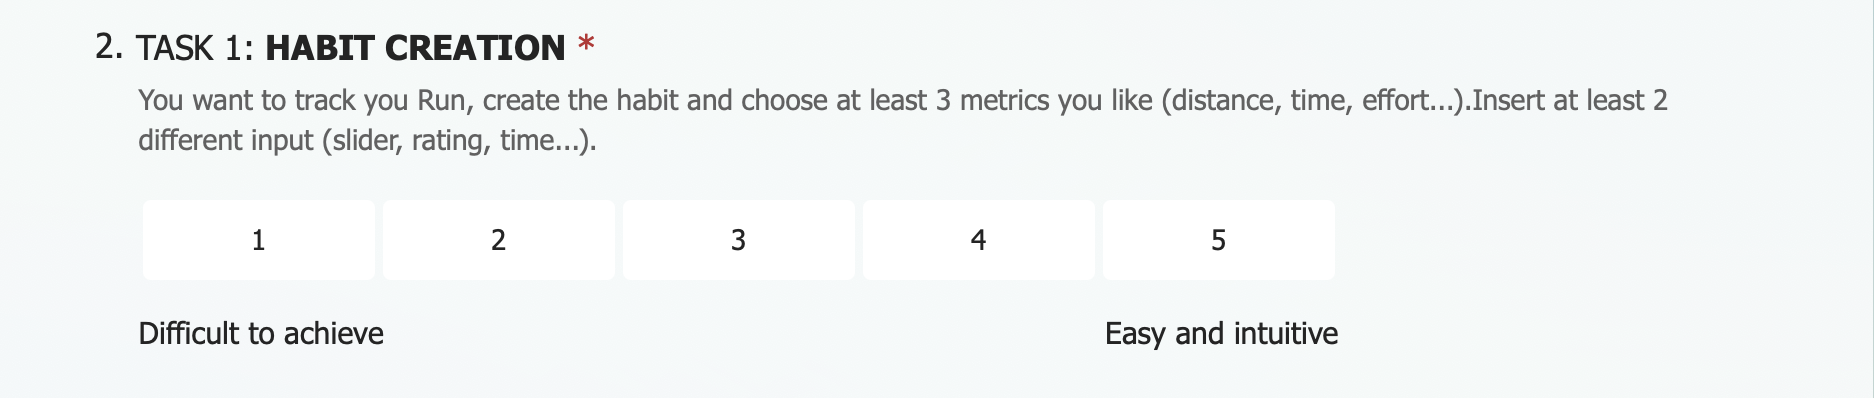
\includegraphics[width=\linewidth]{images/habit_creation.png}
\end{center}

\subsection{Task 2: Habit logging with vocal assistant}
\ititle{Description:} The user is asked to log a habit using the voice assistant. This task assesses how easily the user can use voice commands to log habits without needing to enter data manually.
\\
\ititle{Question}
\begin{center}
	  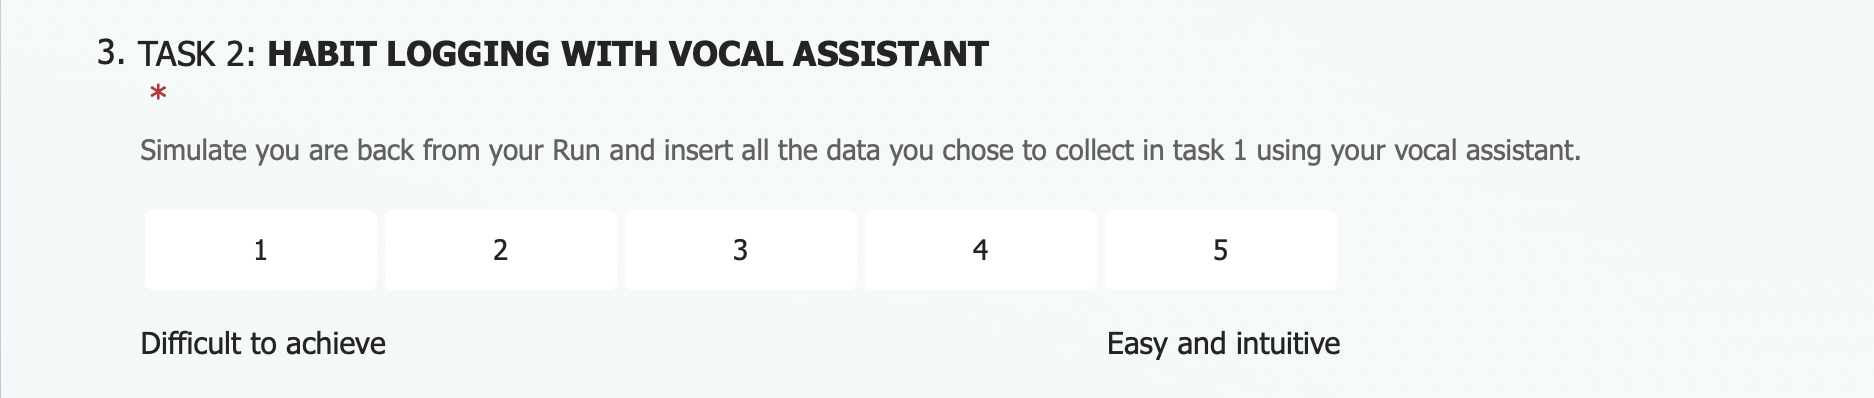
\includegraphics[width=\linewidth]{images/habit_logging_va.png}
\end{center}

\subsection{Task 3: Health from Apple}
\ititle{Description:} The user is asked to connect the app with Apple Health and retrieve health data. This task tests the user’s ability to integrate external health data into the app.
\\
\ititle{Question}
\begin{center}
	  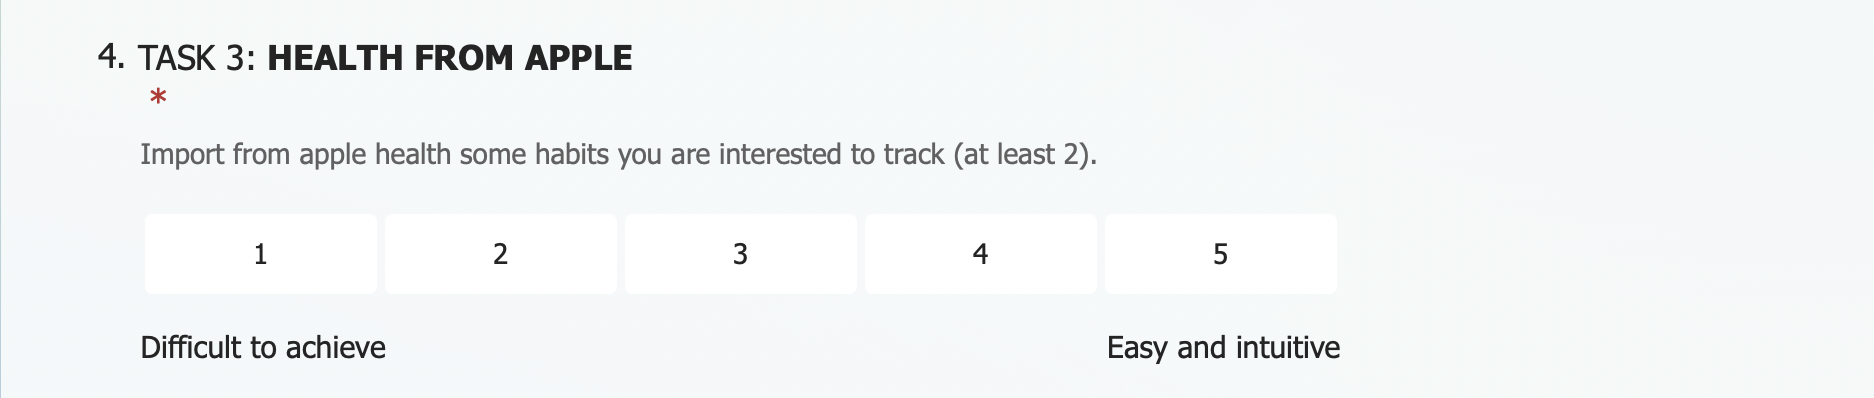
\includegraphics[width=\linewidth]{images/apple_health.png}
\end{center}

\subsection{Task 4: Report creation}
\ititle{Description:} The user is asked to generate a report based on their tracked habits and health metrics. This task evaluates how well the user can review and analyze their progress over time.
\\
\ititle{Question}
\begin{center}
	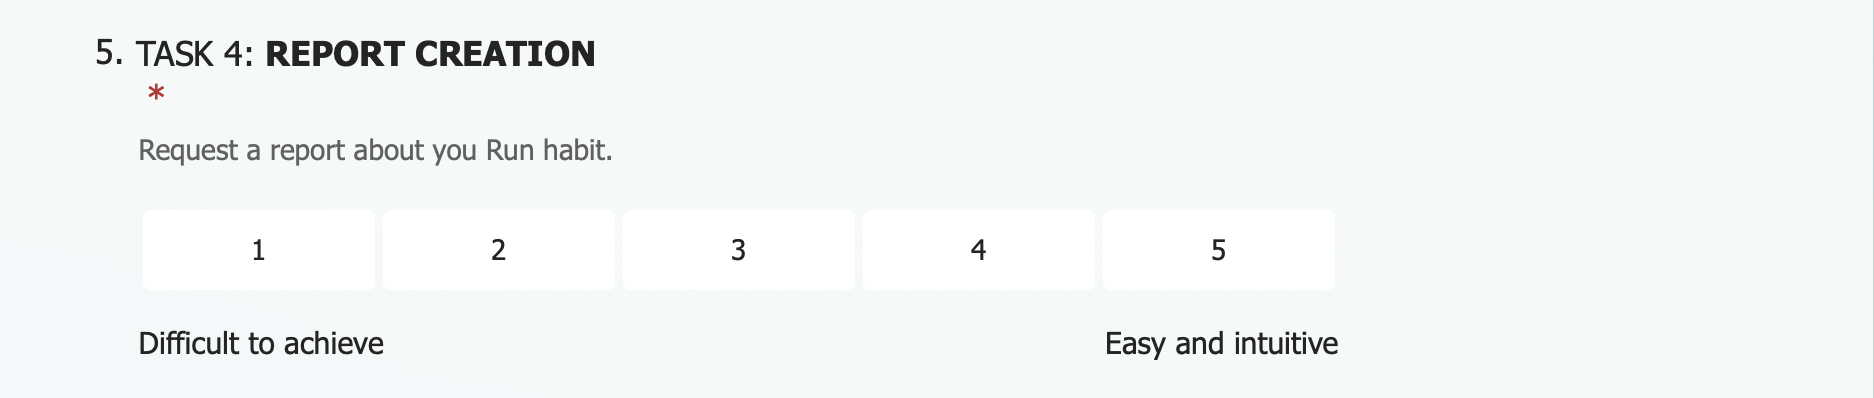
\includegraphics[width=\linewidth]{images/report_creation.png}
\end{center}

\subsection{Task 5: Data visualization}
\ititle{Description:} The user is asked to view visual representations of their habit and health data. This task assesses the user's ability to interpret charts and graphs to understand their progress.
\\
\ititle{Question}
\begin{center}
	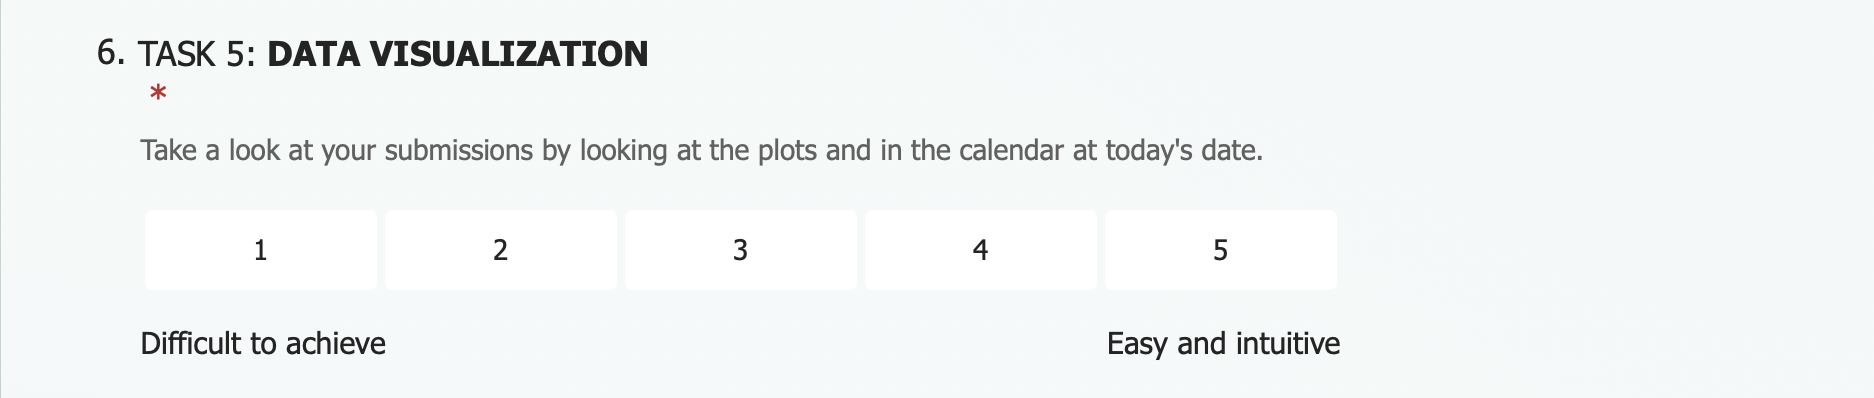
\includegraphics[width=\linewidth]{images/data_visualization.png}
\end{center}

\subsection{Task 6: Removing data}
\ititle{Description:} The user is asked to delete a habit along with its associated data. This task checks how effectively the user can manage and remove personal data from the app.
\\
\ititle{Question}
\begin{center}
	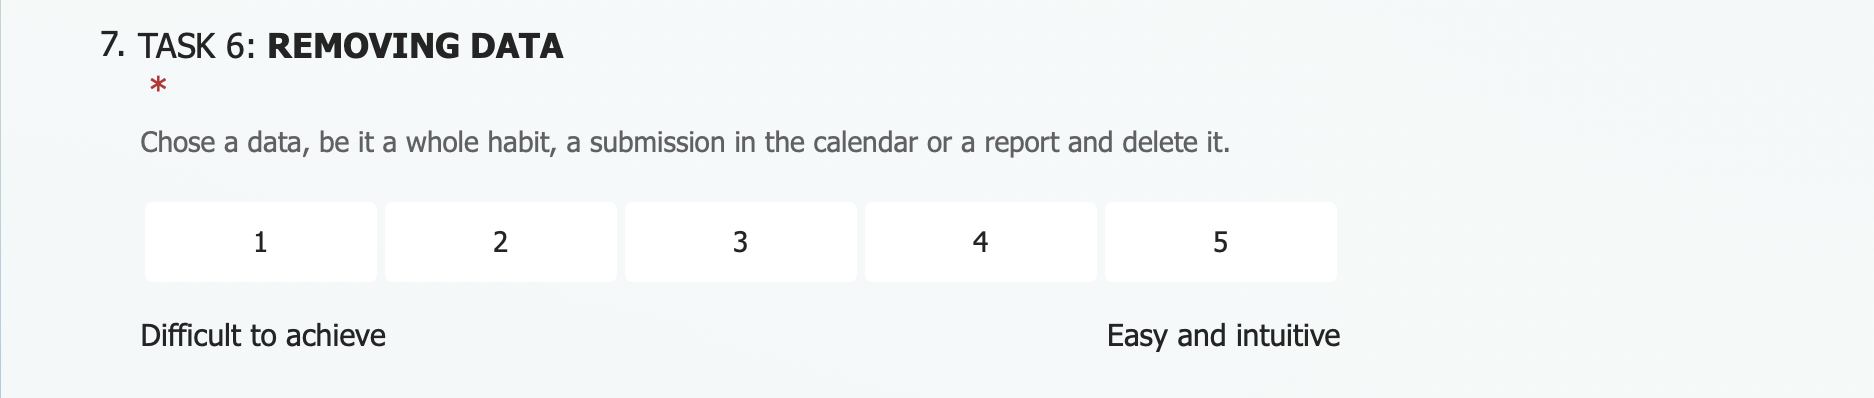
\includegraphics[width=\linewidth]{images/data_removal.png}
\end{center}

\section{Results analysis}
The results of the user testing are summarized in the following sections, which include the average difficulty rating for each task.
\subsection{Task 1: Create a new habit}
\begin{center}
  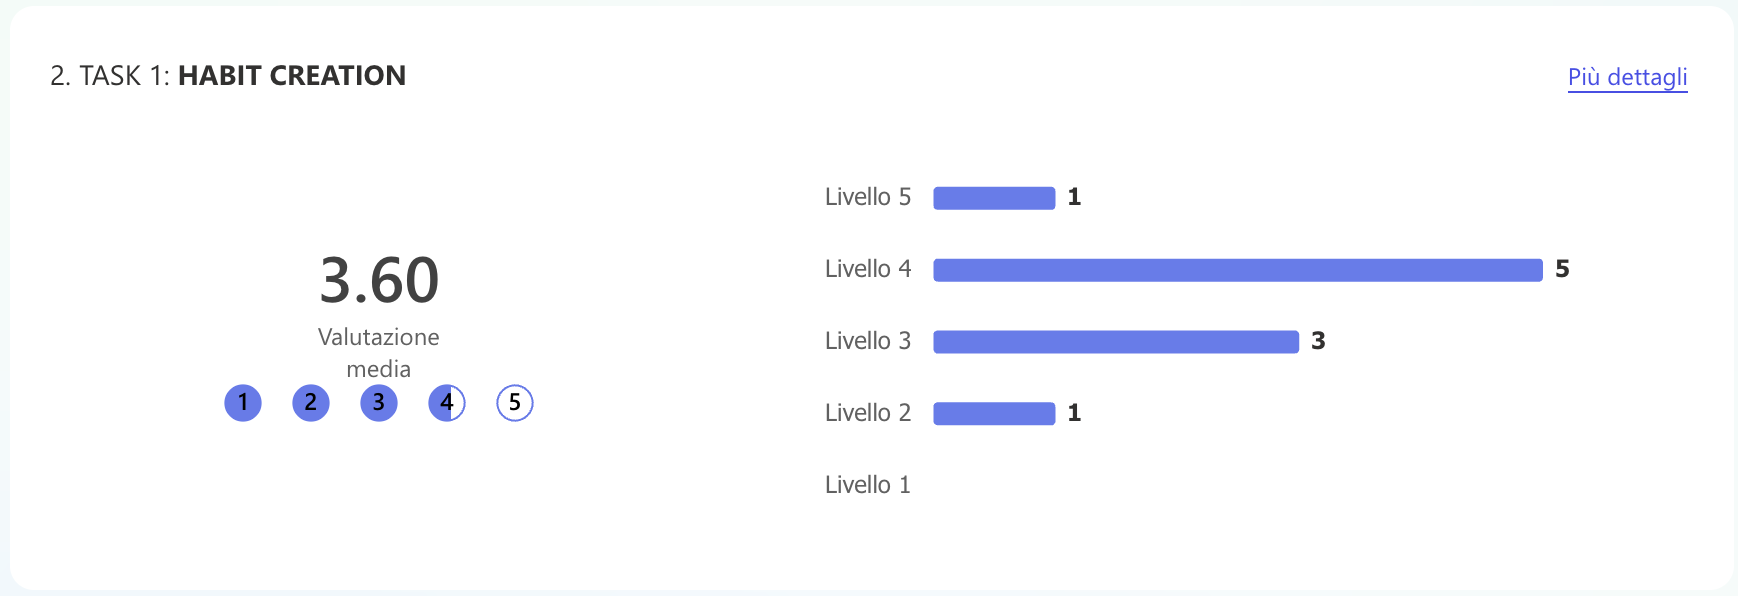
\includegraphics[width=\linewidth]{result_images/habit_creation_result.png}
\end{center}

\subsection{Task 2: Habit logging with vocal assistant}
\begin{center}
  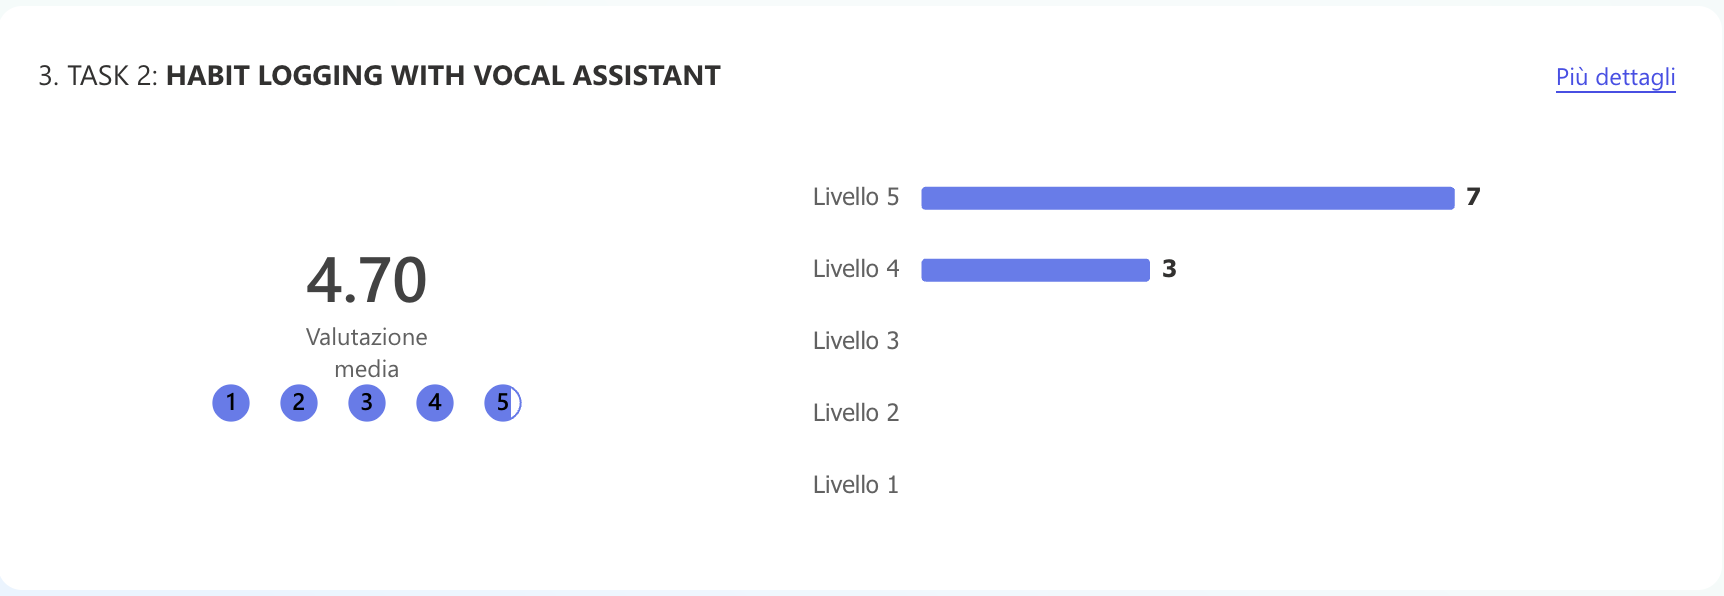
\includegraphics[width=\linewidth]{result_images/habit_logging_with_vocal_result.png}
\end{center}

\subsection{Task 3: Healt from Apple}
\begin{center}
  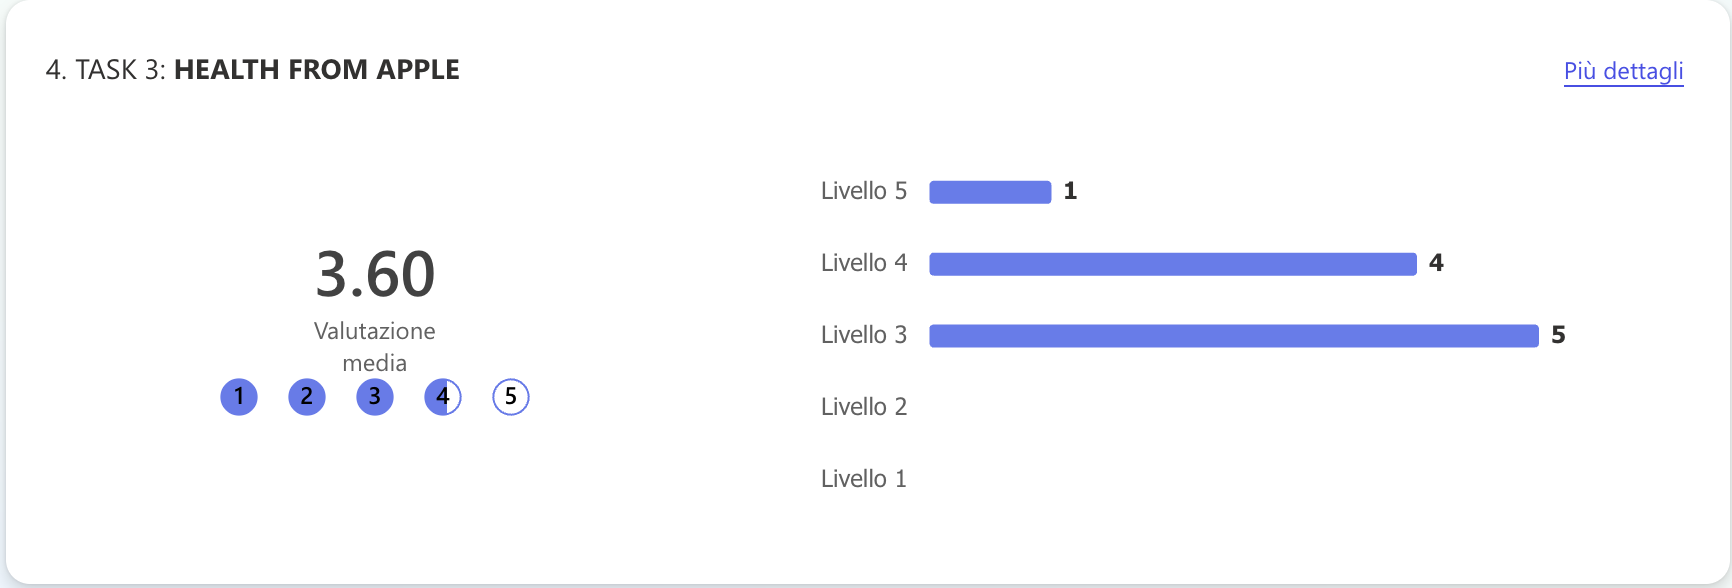
\includegraphics[width=\linewidth]{result_images/helth_from_apple_result.png}
\end{center}

\subsection{Task 4: Report creation}
\begin{center}
  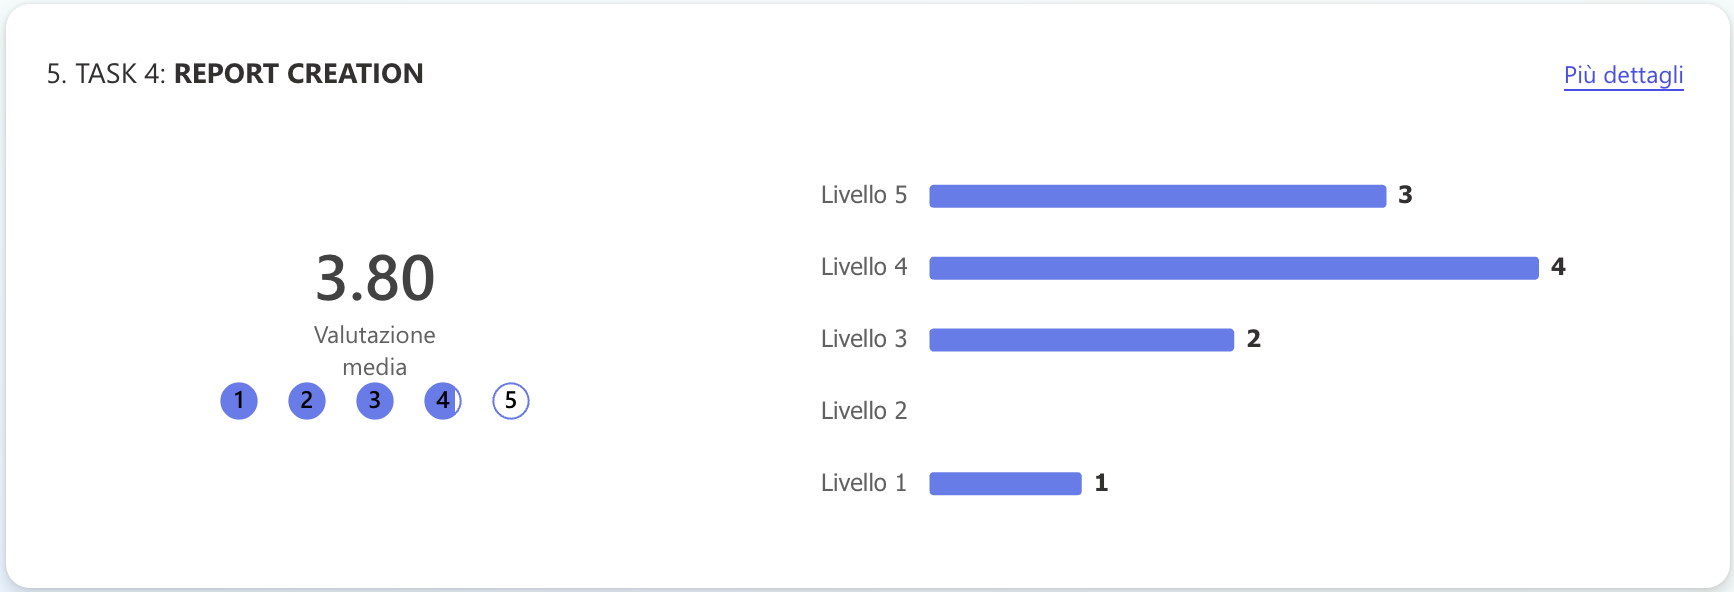
\includegraphics[width=\linewidth]{result_images/report_creation_result.png}
\end{center}

\subsection{Task 5: Data visualization}
\begin{center}
  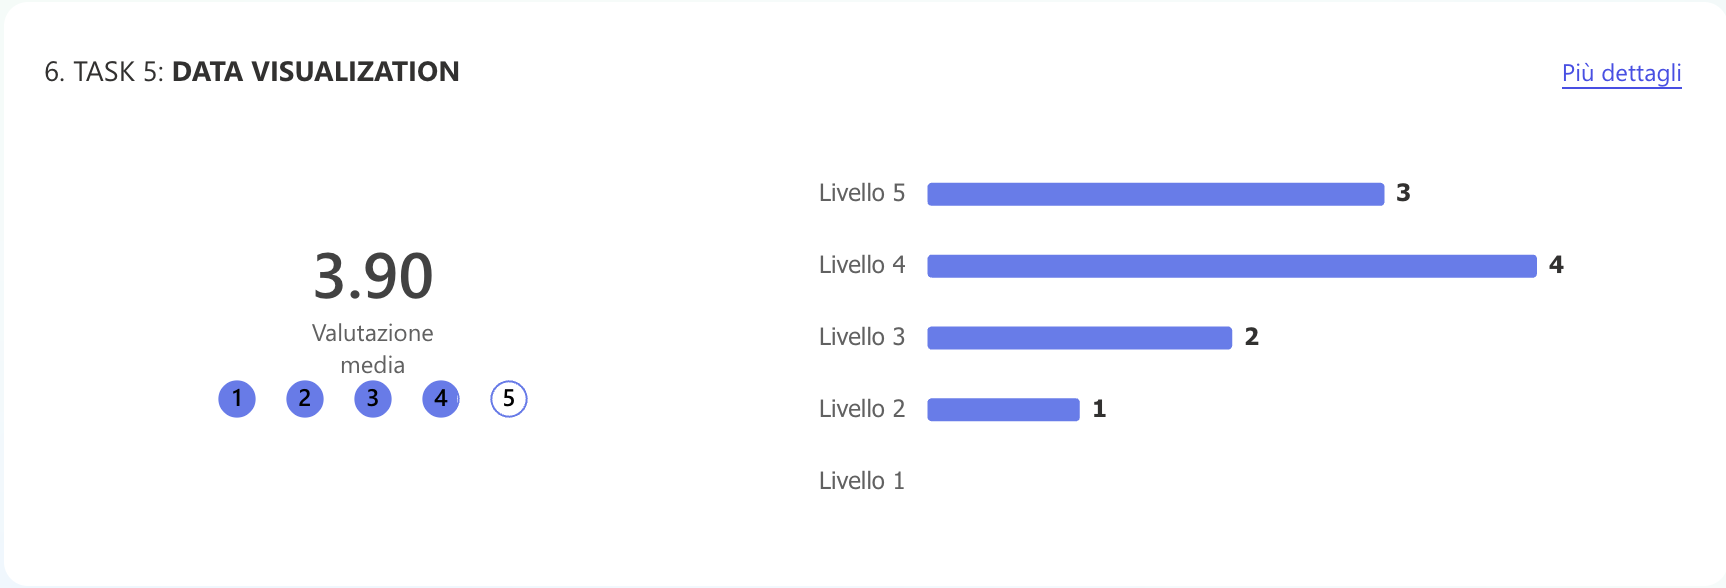
\includegraphics[width=\linewidth]{result_images/data_visualization_result.png}
\end{center}

\subsection{Task 6: Removing data}
\begin{center}
  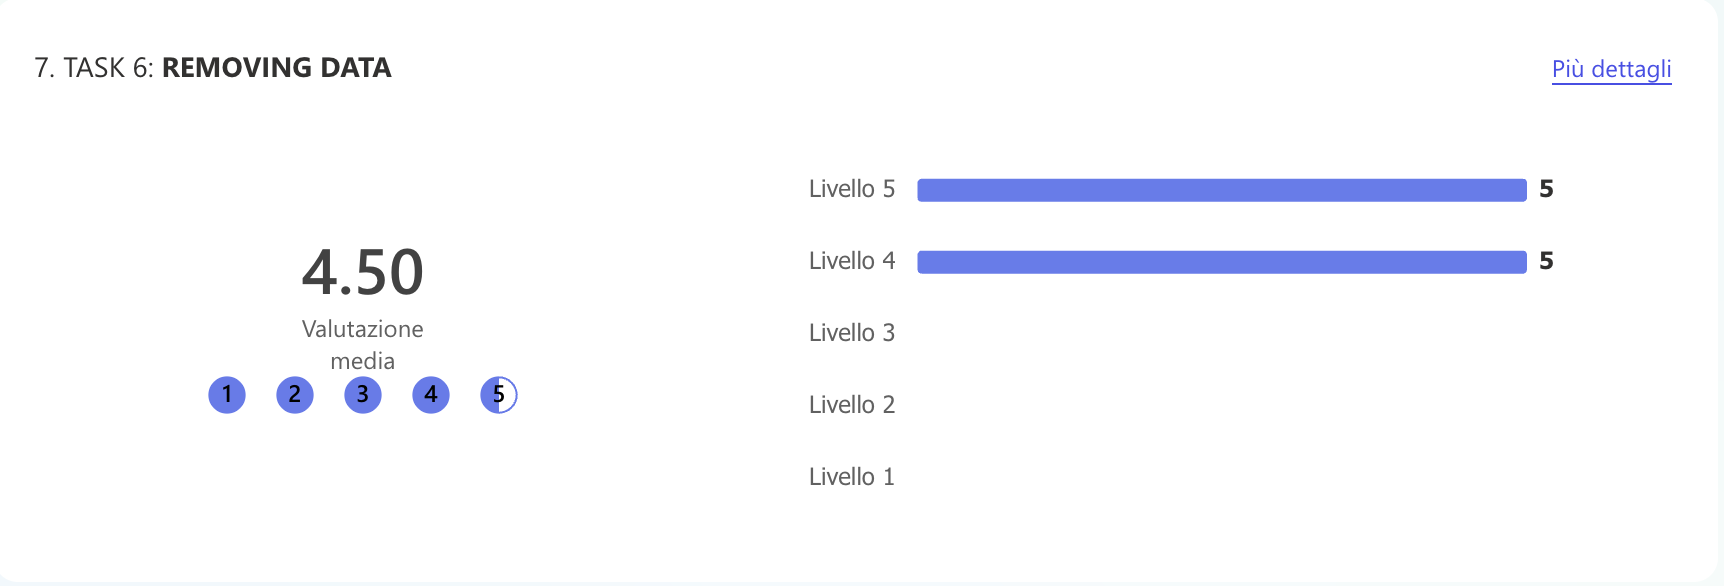
\includegraphics[width=\linewidth]{result_images/remove_habit_result.png}
\end{center}

\section{Suggested improvements}
Here we show the textual feedback received in the form.
\begin{itemize}
	\item I think the application is very well-made: the features are well-distributed, the colors are "in line" with the main concept, and it has everything needed to fulfill its purpose. However, I encountered several problems. During the creation phase, some metrics are counterintuitive, and certain data, like goals, can only be set at the beginning and therefore aren't modifiable during normal use. In general, I think being able to modify a habit could be convenient (for example, if you realize a spelling error only after adding progress). The statistics phase, however, is perfect. The data import phase is very useful, but I think it could be improved regarding the actual import of activity. That is, when I first import an activity, I expect it to automatically import all data up to that moment; it's obvious then that if there are updates I want to include, I'll have to do that manually. The report phase, however, is very well done.
	\item I found the delete function quick and convenient, as well as the ability to import data from Apple Health. I would have liked to manage habit entry directly from the calendar.
	\item I would have preferred to have the week selection below the data visualization because the arrows get confused with the arrows for changing the data being displayed. Additionally, it would be better to add dots on the calendar to quickly see if habits were entered on specific days (using different colored dots if two different habits were entered on the same day).
	\item The main page isn't very clear; at first glance, it's hard to understand what each option does. For example, "Import Health" could be "Import Apple Health." On the Import Health page, it's not clear how to upload your data to the app. When creating habits, there's an interactive preview of metrics that I find very confusing for a user who sees an input request and doesn't quite understand what to do with it. I don't understand why you can't enter a number without a slider (I know there's generic text input, but it's not a very intentional option). In the progress page, I find it difficult to visualize which habit, which session, and which metrics are being displayed. I can't think of a good alternative solution right off the bat, but in my opinion, it needs revisiting since I think it's the most important part—to track what you've done well and quickly. I really like the voice feature, even though it's not clear what it's capable of doing and what it's not. In general: the GUI itself isn't bad, but I don't really like the design. The functionalities are nice, but personally, I'd use an app like this primarily for quick tracking and visualization. For voice tracking, we're there, but for visualization, other solutions could be explored.
	\item Make more clear after vocal interation that to have to submit needed a tutorial.
	\item Renaming without doucle click. Form in calendar type null. Highlight date on calendar when submitted. Delete not obvious.
\end{itemize}

\section{General Impressions}

Overall, users find your application \textbf{very well-made} and thoughtfully designed. The \textbf{features are well-distributed}, and the \textbf{color scheme aligns well with the app's core concept}, providing everything needed for its intended purpose.

Specific aspects that received positive feedback include:

\begin{itemize}
    \item \textbf{Effective Statistics and Reports}: The \textbf{statistics and report sections are considered perfect and very well done}, indicating strong performance in data analysis and presentation.
    \item \textbf{Convenient Deletion and Data Import}: The \textbf{delete function is quick and convenient}, and the ability to \textbf{import data from Apple Health is highly appreciated} and deemed very useful.
    \item \textbf{Promising Voice Feature}: The \textbf{voice functionality is liked}, showing potential for efficient interaction, particularly for quick tracking.
\end{itemize}

\section{Areas for Improvement}

While the app has many strengths, several areas could be refined to enhance the user experience:

\subsection{Onboarding and Clarity}

\begin{itemize}
    \item \textbf{Main Page Clarity}: The \textbf{main page isn't immediately clear}, making it hard for new users to understand what each option does. Renaming options, such as "Import Health" to "Import Apple Health," could help.
    \item \textbf{Data Import Process}: The process for \textbf{uploading data on the "Import Health" page needs to be clearer}. Additionally, users expect the app to \textbf{automatically import historical data} when an activity is first imported, rather than only current data.
\end{itemize}

\subsection{Habit Creation and Management}

\begin{itemize}
    \item \textbf{Habit Modification}: Users desire the ability to \textbf{modify habits after creation} (e.g., correcting spelling errors) to ensure accuracy over time.
    \item \textbf{Confusing Interactive Preview}: The \textbf{interactive preview of metrics during habit creation is confusing}; users don't understand the purpose of the input requested.
\end{itemize}

\subsection{Visualization and Navigation}

\begin{itemize}
    \item \textbf{Calendar Integration}: Users would like to \textbf{manage habit entry directly from the calendar}.
    \item \textbf{Calendar Visual Cues}: Adding \textbf{colored dots to the calendar} to quickly visualize habit entries on specific days (and distinguishing between multiple habits on the same day) would greatly improve glanceability.
    \item \textbf{Week Selection Confusion}: The \textbf{week selection arrows on data visualization pages are confusing}, often mistaken for data change arrows. Moving the week selection below the data visualization could resolve this.
\end{itemize}


This feedback suggests a strong foundation for your app, with clear opportunities to enhance user intuition, flexibility, and visual clarity, especially in habit management and data presentation.

\end{document}
